%================================================================
% SLO
%----------------------------------------------------------------
% datoteka: 	thesis_template.tex
%
% opis: 		predloga za pisanje diplomskega dela v formatu LaTeX na
% 				Univerza v Ljubljani, Fakulteti za računalništvo in informatiko
%
% pripravili: 	Matej Kristan, Zoran Bosnić, Andrej Čopar,
%			  	po začetni predlogi Gašperja Fijavža
%
% popravil: 	Domen Rački, Jaka Cikač, Matej Kristan
%
% verzija: 		30. september 2016 (dodan razširjeni povzetek)
%================================================================


%================================================================
% SLO: definiraj strukturo dokumenta
% ENG: define file structure
%================================================================
\documentclass[a4paper, 12pt]{book}

%================================================================
% SLO: Odkomentiraj "\SLOtrue " za izbiro slovenskega jezika
% ENG: Uncomment "\SLOfalse" to chose English languagge
%================================================================
\newif\ifSLO
% switch language

\SLOtrue % Enables Slovenian language
%\SLOfalse  % Enables English language

%================================================================
% SLO: vključi oblikovanje in pakete
% ENG: include design and packages
%================================================================
%----------------------------------------------------------------
% SLO: LaTeX paketi
% ENG: LateX packages
%----------------------------------------------------------------
% SLO: omogoča uporabo slovenskih (latinskih) črk kodiranih v formatu UTF-8
% ENG: enables the use of slovene (latin) caracters encoded in the UFT-8 format
\usepackage[utf8x]{inputenc}
%\inputencoding{utf8} 
% SLO: naloži, med drugim, slovenske delilne vzorce
% ENG: loads, among others, slovene dividing patterns
\usepackage[slovene,english]{babel} 
% SLO: poskrbi za postavitev strani
% ENG: takes care of the page layout
\usepackage{fancyhdr}
% SLO: za vlaganje slik različnih formatov
% ENG: for loading figures of different formats
\usepackage{graphicx}
\usepackage{caption}
\captionsetup[figure]{labelfont=bf} % SLO: napis "Slika #" v krepkem tisku
									% ENG: wirte "Figure #" caption in bold
\captionsetup[table]{labelfont=bf} % SLO: napis "Tabela #" v krepkem tisku
								   % ENG: wirte "Table #" caption in bold

% SLO: za pisanje psevdokode
% ENG: for writing pseudocode
\usepackage{algorithm}
\usepackage{algorithmic}
\floatname{algorithm}{\footnotesize Algorithm} % SLO: napis "Algoritem #" v krepkem tisku
											   % ENG: write "Algorithm #" caption in bold
% SLO: poveže reference slik/tabel in slike/tabele znotraj dokumenta
% ENG: links image/table references with the images/tables within the document
\usepackage{hyperref}
% SLO: pri kliku na referenco slike/tabele se postavi na vrh slike/tabele
% ENG: when clicking the image/table reference, position the focus on top of the image/table
\usepackage[all]{hypcap}
% SLO: omogoča, med drugim, definicjo in uporebo barve
% ENG: enables, among others, the definition and use of colors
\usepackage{xcolor}
%----------------------------------------------------------------
% SLO: dodatni paketi
% ENG: additional packages
%----------------------------------------------------------------
% SLO: omogoča večjo manipulacijo nad tabelami
% ENG: allows for greater manipulation of tables
\usepackage{booktabs}
% SLO: naloži dodatne simbole
% ENG: loads additional symbols
\usepackage{amssymb} 
% SLO: omogoča, med drugim, sklicevanje na formule z eqref
% ENG: enables, among others, equation referencing with eqref
\usepackage{amsmath}
% SLO: omogoča komentiranje večjega dela teksta
% ENG: enables the commenting of larger text parts
\usepackage{verbatim}
% SLO: omogoča rotacijo PDF strani v ležeč položaj
% ENG: enables the rotation of a PDF page to landscape
\usepackage{pdflscape}
% SLO: omogoča barvanje vrstic in stolpcev tabel
% ENG: enables coloring of table rows and columns
\usepackage{colortbl}

\usepackage{url}


%================================================================
% SLO: nastavitve dokumenta
% ENG: document properties
%================================================================
% SLO: prilagoditev robov za tisk
% ENG: margin adjustments for printing
\addtolength{\marginparwidth}{-20pt}
\addtolength{\oddsidemargin}{40pt}
\addtolength{\evensidemargin}{-40pt}
% SLO: razmik med vrsticami
% ENG: line spacing
\renewcommand{\baselinestretch}{1.3} 
% SLO: postavitev strani
% ENG: page layout
\renewcommand{\chaptermark}[1]{\markboth{\MakeUppercase{\thechapter.\ #1}}{}} 
\renewcommand{\sectionmark}[1]{\markright{\MakeUppercase{\thesection.\ #1}}} 
\renewcommand{\headrulewidth}{0.5pt} % Header rule
\renewcommand{\footrulewidth}{0pt} % Footer rule
%
\fancypagestyle{frontmatter}{%
	\fancyhf{} % Clear all headers and footers first
	\fancyhead[LE, RO]{\sl \thepage} 
	%\fancyhead[LO]{\sl \rightmark} 
	%\fancyhead[RE]{\sl \leftmark}
}
\fancypagestyle{mainmatter}{%
  	\fancyhf{} % Clear all headers and footers first
	\fancyhead[LE,RO]{\sl \thepage} 
	\fancyhead[LO]{\sl \rightmark} 
	\fancyhead[RE]{\sl \leftmark}
}
% SLO: font za ime avtorja
% ENG: font for author name
\newcommand{\authorfont}{\Large}
% SLO: font za naslov diplomskega dela
% ENG: font for thesis title
\newcommand{\titlefont}{\LARGE\bf}
% SLO: globina kazala
% ENG: content depth
\setcounter{tocdepth}{1}
% SLO: definiraj ukaz za prazno stran
% ENG: define the command for empty page
\newcommand{\clearemptydoublepage}{\newpage{\pagestyle{empty}\cleardoublepage}}

\newcommand{\BibTeX}{{\sc Bib}\TeX}


%----------------------------------------------------------------
% |||||||||||||||||||||| USTREZNO POPRAVI |||||||||||||||||||||||
% |||||||||||||||||||||| EDIT ACCORDINGLY |||||||||||||||||||||||
%----------------------------------------------------------------
\newcommand{\ttitle}{Barvanje črnobelih slik z globokimi modeli}
\newcommand{\ttitleEn}{Deep models for image coloring}
\newcommand{\tsubject}{\ttitle}
\newcommand{\tsubjectEn}{\ttitleEn}
\newcommand{\tauthor}{Primož Godec}
\newcommand{\temail}{p.godec9@gmail.com}
\newcommand{\myyear}{2017}
\newcommand{\tkeywords}{Umetna inteligenca, Odkiravanje znanj iz podatkov, globoko učenje, nevronske mreže}
\newcommand{\tkeywordsEn}{Artificial inteligence, data mining, deep learning, neural networks}
\newcommand{\mysupervisor}{prof.~dr.~Blaž Zupan}
\newcommand{\mycosupervisor}{}

% include formatted front pages

%----------------------------------------------------------------
% SLO: definiraj metapodatke za datoteko thesis_template.tex
% ENG: define metadata for the file thesis_template.tex
%----------------------------------------------------------------
%----------------------------------------------------------------
%	HYPERREF SETUP
% SLO: ustrezno popravi e-mail
% ENG: edit the e-mail accordingly
%----------------------------------------------------------------
\hypersetup{pdftitle={\ttitle}}
\hypersetup{pdfsubject=\ttitleEn}
\hypersetup{pdfauthor={\tauthor, \temail}}
\hypersetup{pdfkeywords=\tkeywordsEn}

%----------------------------------------------------------------
% define medatata
% SLO: ustrezno popravi e-mail
% ENG: edit the e-mail accordingly
%----------------------------------------------------------------
\def\Title{\ttitle}
\def\Author{\tauthor, \temail}
\def\Subject{\ttitleEn}
\def\Keywords{\tkeywordsEn}
\def\Org{Univerza v Ljubljani, Fakulteta za računalništvo in informatiko}

%%%%%%%%%%%%%%%%%%%%%%%%%%%%%%%%%%%%%%%%
% \convertDate converts D:20080419103507+02'00' to 2008-04-19T10:35:07+02:00
%%%%%%%%%%%%%%%%%%%%%%%%%%%%%%%%%%%%%%%%
\def\convertDate{%
    \getYear
}

{\catcode`\D=12
 \gdef\getYear D:#1#2#3#4{\edef\xYear{#1#2#3#4}\getMonth}
}
\def\getMonth#1#2{\edef\xMonth{#1#2}\getDay}
\def\getDay#1#2{\edef\xDay{#1#2}\getHour}
\def\getHour#1#2{\edef\xHour{#1#2}\getMin}
\def\getMin#1#2{\edef\xMin{#1#2}\getSec}
\def\getSec#1#2{\edef\xSec{#1#2}\getTZh}
\def\getTZh +#1#2{\edef\xTZh{#1#2}\getTZm}
\def\getTZm '#1#2'{%
    \edef\xTZm{#1#2}%
    \edef\convDate{\xYear-\xMonth-\xDay T\xHour:\xMin:\xSec+\xTZh:\xTZm}%
}

\expandafter\convertDate\pdfcreationdate


%%%%%%%%%%%%%%%%%%%%%%%%%%%%%%%%%%%%%%%%
% get pdftex version string
%%%%%%%%%%%%%%%%%%%%%%%%%%%%%%%%%%%%%%%%
\newcount\countA
\countA=\pdftexversion
\advance \countA by -100
\def\pdftexVersionStr{pdfTeX-1.\the\countA.\pdftexrevision}

%%%%%%%%%%%%%%%%%%%%%%%%%%%%%%%%%%%%%%%%
% XMP data
%%%%%%%%%%%%%%%%%%%%%%%%%%%%%%%%%%%%%%%%
\usepackage{xmpincl}

%%%%%%%%%%%%%%%%%%%%%%%%%%%%%%%%%%%%%%%%
% pdfInfo
%%%%%%%%%%%%%%%%%%%%%%%%%%%%%%%%%%%%%%%%
\pdfinfo{%
    /Title    (\ttitle)
    /Author   (\tauthor, \temail)
    /Subject  (\ttitleEn)
    /Keywords (\tkeywordsEn)
    /ModDate  (\pdfcreationdate)
    /Trapped  /False
}

%================================================================
% SLO: razno
% ENG: other
%================================================================
% SLO: nastavitev sklicevanj
% ENG: hyper referencing setup
\definecolor{black}{rgb}{0,0,0}
\hypersetup{
	colorlinks = true,
	linkcolor = black,
	citecolor = black,
	urlcolor = black
}

%----------------------------------------------------------------
% SLO: dodaj poti do datotek s slikami, tabelami, ...
% ENG: add paths to files containing figures, tables, ...
%----------------------------------------------------------------
\graphicspath{
	{./figures/}
	{./tables/}
}
%----------------------------------------------------------------
% SLO: moji paketi
% ENG: my packages
%----------------------------------------------------------------
% ...
%----------------------------------------------------------------
% SLO: moji konstrukti
% ENG: my constructs
%----------------------------------------------------------------
\newtheorem{izrek}{Izrek}[chapter]
\newtheorem{trditev}{Trditev}[izrek]
\newenvironment{dokaz}{\emph{Dokaz.}\ }{\hspace{\fill}{$\Box$}}


%================================================================
% SLO: začetne strani magistrskega dela
% ENG: fist pages of the master's thesis
%================================================================
\begin{document}
% SLO: prepreči težave s številkami strani v kazalu
% ENG: prevents problems with the page numbers in the contents page
\renewcommand{\thepage}{}

%----------------------------------------------------------------
% Language-dependent formatting
%----------------------------------------------------------------
\ifSLO
    % SLO: naslovnica (vstavi naslovnico (LaTeX kodo) iz datoteke pages/title.tex)
    \thispagestyle{empty}
	\begin{center}
        {\large\sc Univerza v Ljubljani\\Fakulteta za računalništvo in informatiko}
    	\vskip 10em
    	{\authorfont \tauthor \par}
    	{\titlefont \ttitle \par}
    {\vskip 2em \textsc{MAGISTRSKO DELO\\[2mm]
    MAGISTRSKI PROGRAM DRUGE STOPNJE\\RAČUNALNIŠTVO IN INFORMATIKA}\par}
    \vfill\null
    {\large \textsc{Mentor}: \mysupervisor \par}
   	%{\large \textsc{Somentor}: \mycosupervisor \par}
    {\vskip 2em \large Ljubljana, \myyear \par}
\end{center} \clearemptydoublepage
    % SLO: avtorske pravice
    \thispagestyle{empty}
\vspace*{\fill}
{\noindent\footnotesize
{\sc Avtorske pravice}. Rezultati magistrskega dela so intelektualna lastnina avtorja in Fakultete za ra\-ču\-nal\-niš\-tvo in informatiko Univerze v Ljubljani. Za objavljanje ali izkoriščanje rezultatov ma\-gi\-str\-ske\-ga dela je potrebno pisno soglasje avtorja, Fakultete za ra\-ču\-nal\-niš\-tvo in informatiko ter mentorja.}
\begin{center}
{\footnotesize{\sc \copyright \myyear\ \tauthor}}
\end{center} \clearemptydoublepage
    % SLO: izjava o avtorstvu (ni več del vezane izdaje, ločena oddaja)
    % SLO: zahvala
    \thispagestyle{empty}

\begin{center}
{\Large \textbf{\sc Zahvala}}
\end{center}
\vspace{0.5cm}

{\it\noindent
Na tem mestu zapišite, komu se zahvaljujete za izdelavo magistrske naloge. V zahvali se poleg mentorja spodobi omeniti vse, ki so s svojo pomočjo prispevali k nastanku vašega izdelka.

\vspace{0.5cm} \hfill \tauthor, \myyear
} \clearemptydoublepage
    % SLO: posvetilo
    \thispagestyle{empty}\mbox{}{\vskip0.20\textheight}\mbox{}\hfill\begin{minipage}{0.55\textwidth}%

Ani.\\\\
\textit{''In nature, light creates the color. In the picture, color creates the light.''}
\flushright --- Hans Hofmann
\normalfont\end{minipage} \clearemptydoublepage
\else
    % ENG: title page (insert the title page (LaTeX code) from the file pages/title.tex)
    \thispagestyle{empty}
	\begin{center}
        {\large\sc University of Ljubljana\\Faculty of Computer and Information Science}
    	\vskip 10em
    	{\authorfont \tauthor \par}
    	{\titlefont \ttitleEn \par}
    {\vskip 2em \textsc{MASTER'S THESIS\\[2mm]
    THE 2nd CYCLE MASTER'S STUDY PROGRAMME\\COMPUTER AND INFORMATION SCIENCE}\par}
    \vfill\null
    {\large \textsc{Supervisor}: \mysupervisor \par}
   	{\large \textsc{Co-supervisor}:  \mycosupervisor \par}
    {\vskip 2em \large Ljubljana, \myyear \par}
\end{center}\thispagestyle{empty}
	\begin{center}
        {\large\sc University of Ljubljana\\Faculty of Computer and Information Science}
    	\vskip 10em
    	{\authorfont \tauthor \par}
    	{\titlefont \ttitleEn \par}
    {\vskip 2em \textsc{MASTER'S THESIS\\[2mm]
    THE 2nd CYCLE MASTER'S STUDY PROGRAMME\\COMPUTER AND INFORMATION SCIENCE}\par}
    \vfill\null
    {\large \textsc{Supervisor}: \mysupervisor \par}
   	{\large \textsc{Co-supervisor}:  \mycosupervisor \par}
    {\vskip 2em \large Ljubljana, \myyear \par}
\end{center}\include{title_page.tex}   \clearemptydoublepage
    % ENG: copyright
    \thispagestyle{empty}
\vspace*{\fill}
{\noindent\footnotesize
{\sc Copyright}. The results of this master's thesis are the intellectual property of the author and the Faculty of Computer and Information Science, University of Ljubljana. For the publication or exploitation of the master's thesis results, a written consent of the author, the Faculty of Computer and Information Science, and the supervisor is necessary.}
\begin{center}
{\footnotesize{\sc \copyright \myyear\ \tauthor}}
\end{center}  \clearemptydoublepage
    % ENG: declaration of authorship (not part of paper edition, turn in separately)
    % ENG: acknowledgements
    \thispagestyle{empty}

\begin{center}
{\Large \textbf{\sc Acknowledgments}}
\end{center}
\vspace{0.5cm}

{\it\noindent
Worth mentioning in the acknowledgment is everyone who contributed to your thesis.

\vspace{0.5cm} \hfill \tauthor, \myyear
} \clearemptydoublepage
    % ENG: dedication
    \thispagestyle{empty}\mbox{}{\vskip0.20\textheight}\mbox{}\hfill\begin{minipage}{0.55\textwidth}%

To all the flowers of this world.\\\\
\textit{''The only reason for time is so that everything doesn't happen at once.''}
\flushright --- Albert Einstein
\normalfont\end{minipage} \clearemptydoublepage
\fi

%----------------------------------------------------------------
% SLO: kazalo
% ENG: contents
%----------------------------------------------------------------
\begingroup
	\hypersetup{colorlinks=true,linkcolor=black}
	\def\thepage{}
	\tableofcontents{}
	\clearemptydoublepage
\endgroup


%\ifSLO
%    % SLO: seznam kratic
%    \chapter*{Seznam uporabljenih kratic}

\begin{tabular}{l|l|l}
  {\bf kratica} & {\bf angleško} & {\bf slovensko} \\ \hline
  % after \\: \hline or \cline{col1-col2} \cline{col3-col4} ...
  {\bf CA} & classification accuracy & klasifikacijska točnost \\
  {\bf DBMS} & database management system & sistem za upravljanje podatkovnih baz \\
  {\bf SVM} & support vector machine & metoda podpornih vektorjev \\
  ... & ... & ... \\
\end{tabular} \clearemptydoublepage
%    % SLO: glavne strani diplomskega dela
%\else
%    % ENG: list of acronmys
%    \chapter*{List of used acronmys}

\begin{tabular}{l|l|l}
  {\bf acronym} & {\bf meaning}  \\ \hline
  % after \\: \hline or \cline{col1-col2} \cline{col3-col4} ...
  {\bf CA} & classification accuracy \\
  {\bf DBMS} & database management system \\
  {\bf SVM} & support vector machine \\
  ... & ... \\
\end{tabular} \clearemptydoublepage
%\fi

\frontmatter
\pagestyle{frontmatter}
\setcounter{page}{1} %
\renewcommand{\thepage}{}       % preprecimo težave s številkami strani v kazalu


% include Slovenian abstract
%---------------------------------------------------------------
% SLO: slovenski povzetek
% ENG: slovenian abstract
%---------------------------------------------------------------
\selectlanguage{slovene} % Preklopi na slovenski jezik
\addcontentsline{toc}{chapter}{Povzetek}
\chapter*{Povzetek}

\noindent\textbf{Naslov:} \ttitle
\bigskip

Barvna fotografija je prišla v vsakdanjo uporabo šele v zadnjih 50 letih, zato so razni arhivi polni črno-belih fotografij, katere bi njihovi lastniki radi obarvali. V ta namen so bili razviti različni algoritmični pristopi.
V disertaciji predstavljamo nekaj novih avtomatskih pristopov za barvanje črno-belih slik in videov, ki so osnovani na konvolucijskih nevronskih mrežah. Pristope primerjamo s pristopi iz sorodnih del in jih preizkusimo na starih črno-belih slikah. 
Iz rezultatov je razvidno, da naši pristopi dosegajo kvaliteto barvanja pristopov iz sorodnih del. Naš nov pristop, ki obarva slike po delih, pa izboljša barvanje slik velikosti, ki so različne od tistih, na katerih je bila mreža naučena. Ta pristop je tudi naučen hitreje kot pristopi na celih slikah. 

\subsection*{Ključne besede}
\textit{\tkeywords}
\clearemptydoublepage
% include English abstract
 %---------------------------------------------------------------
% SLO: angleški povzetek
% ENG: english abstract
%---------------------------------------------------------------
\selectlanguage{english} % Preklopi na angleški jezik
\addcontentsline{toc}{chapter}{Abstract}
\chapter*{Abstract}

\noindent\textbf{Title:} \ttitleEn
\bigskip

Because the color photography came in everyday use in last fifty years our grandparents are still owning many black and white photographs which they like to look at to remember the old times. It is more pleasant to look at photos with some colors than a black and white one, they also look more natural. It encourages researchers to develop approaches for black and white photographs and video colorization.

In this thesis we present new approaches for automatic black and white photo colorization based on convolutional neural networks which are working on parts of images instead of taking into account full image. That approaches allows us to color images of different size to those used for training with almost equal accuracy. We also present comparison between our own approaches and those presented in related works. 


\subsection*{Keywords}
\textit{\tkeywordsEn}
\clearemptydoublepage

% Include extended abstract [Razširjeni povzetek v slovenščini-- le za dela pisana v angleščini]
\ifSLO
\else
  %  \cleardoublepage
    \let\oldthesection=\thesection %Special section numbering for this chapter - remember default one
    \let\oldthesubsection=\thesubsection
    \renewcommand{\thesection}{\Roman{section}} %Special section numbering for this chapter
    \renewcommand{\thesubsection}{\thesection.\Roman{subsection}}

    % set roman page numbering
    \pagenumbering{roman}
    % set slovene language
    \selectlanguage{slovene}
    % insert extended abstract
     \chapter{Razširjeni povzetek}
 
 To je primer razširjenega povzetka v slovenščini, ki je obvezen za naloge pisane v angleščini. Razširjeni povzetek mora vsebovati vse glavne elemente dela napisanega v angleščini skupaj s kratkim uvodom in povzetkom glavnih elementov metode, glavnih eksperimentalnih rezultatov in glavnih ugotovitev. Razširjeni povzetek naj bo strukturiran v podpoglavja (spodaj je naveden le okvirni primer in je nezavezujoč).
 Čez palec navadno razširjeni povzetek nanese okoli 10 odstotkov obsega celotnega dela. 
 
 \section{Kratek pregled sorodnih del}
 
 \section{Predlagana metoda}
 
 \section{Eksperimentalna evaluacija}
 
 \section{Sklep}
 
poljuben tekst  poljuben tekst  poljuben tekst  poljuben tekst  poljuben tekst  poljuben tekst  poljuben tekst  poljuben tekst  poljuben tekst  poljuben tekst  poljuben tekst  poljuben tekst  poljuben tekst  poljuben tekst  poljuben tekst  poljuben tekst  poljuben tekst  poljuben tekst  poljuben tekst  poljuben tekst  poljuben tekst  poljuben tekst  poljuben tekst  poljuben tekst  poljuben tekst  poljuben tekst  poljuben tekst  poljuben tekst  poljuben tekst  poljuben tekst  poljuben tekst  poljuben tekst  poljuben tekst  poljuben tekst  poljuben tekst  poljuben tekst  poljuben tekst  poljuben tekst  poljuben tekst  poljuben tekst  poljuben tekst  poljuben tekst  poljuben tekst  poljuben tekst  poljuben tekst  poljuben tekst  poljuben tekst  poljuben tekst  poljuben tekst  poljuben tekst  poljuben tekst  poljuben tekst  poljuben tekst  poljuben tekst  poljuben tekst  poljuben tekst  poljuben tekst  poljuben tekst  poljuben tekst  poljuben tekst  poljuben tekst  poljuben tekst  poljuben tekst  poljuben tekst  poljuben tekst  poljuben tekst  poljuben tekst  poljuben tekst  poljuben tekst  poljuben tekst  poljuben tekst  poljuben tekst  poljuben tekst  poljuben tekst  poljuben tekst  poljuben tekst  poljuben tekst  poljuben tekst  poljuben tekst  poljuben tekst  poljuben tekst  poljuben tekst  poljuben tekst  poljuben tekst  poljuben tekst  poljuben tekst  poljuben tekst  poljuben tekst  poljuben tekst  poljuben tekst 

 
    \let\thesection=\oldthesection % Restore default section numbering
    \let\thesubsection=\oldthesubsection
\fi

%----------------------------------------------------------------
% SLO: Preklopi izbrani jezik
% ENG: Switch to chosen language
%----------------------------------------------------------------
\ifSLO
    \selectlanguage{slovene} % Preklopi na slovenski jezik
\else
    \selectlanguage{english}  % Switch to english language
\fi

% SLO: vklopi številčenje poglavji, ponastavi številčenje strani in uporabi arabske številkami za številčenje strani
% ENG: turns on chapter numbering, resets page numbering and uses arabic numerals for page numbers
\mainmatter
\pagestyle{mainmatter}
\setcounter{page}{1}
\pagestyle{fancy}


%================================================================
% ENG: main pages of the thesis
%================================================================

%----------------------------------------------------------------
% Poglavje (Chapter) 1: Uvod
%----------------------------------------------------------------
\chapter{Uvod}
\label{ch:uvod}


Algoritmi za barvanje črno-belih slik se uporabljajo na več področjih: barvanje starih slik, barvanje črno-belih filmov in v pomoč pri umetnosti. 
Za človeka je barvanje črno-belih slik, ki so prikazane na sliki \ref{im:pari-cb-b}, enostavna naloga. Z vsakdanjim opazovanjem sveta se je človek naučil, da je nebo modro z belimi oblaki, drevesa so zelena in cesta je siva. Za objekte, ki nimajo enolično določene barve ljudje lahko ugibamo kakšne barve naj bi predmet bil. Pri tem opravilu je potrebno veliko razumevanja, saj iz sivinskih slik ni možno direktno razbrati barv, namreč pri nastanku sivinske slike se veliko informacij izgubi (dve od treh dimenzij).

\begin{figure}
\begin{center}
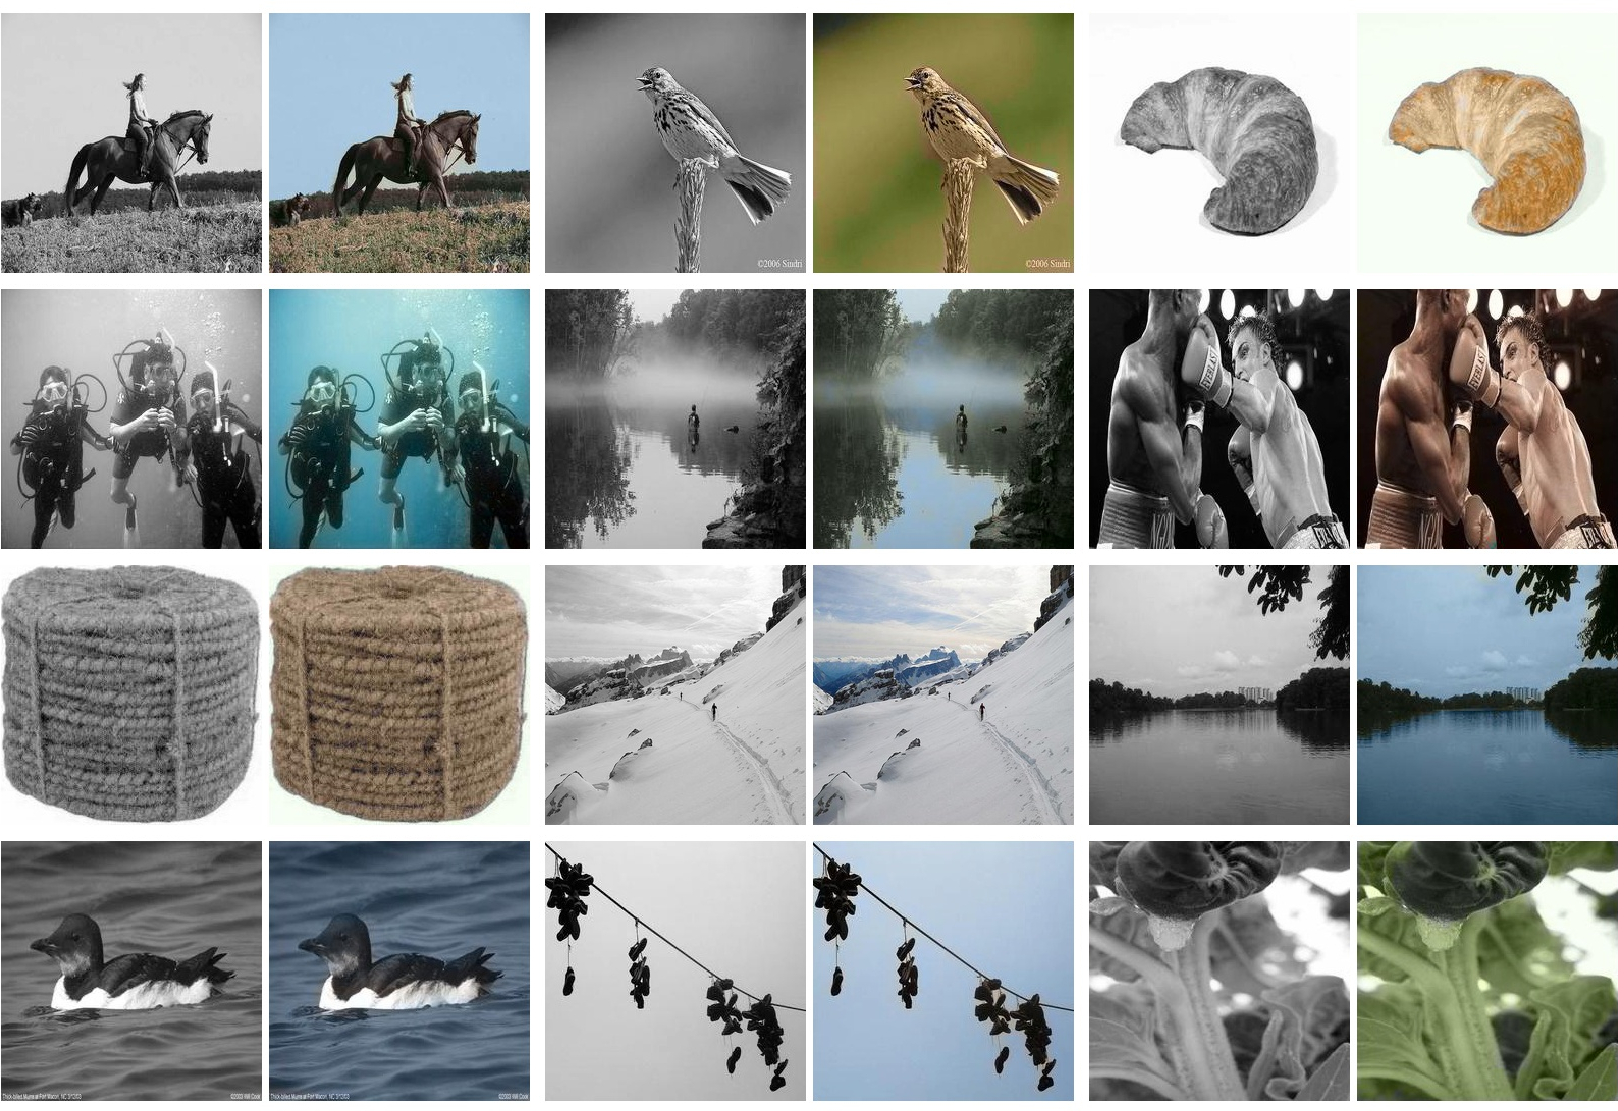
\includegraphics[width=13cm]{black-colored-comparison}
\end{center}
\caption{Primeri barvanja črno-belih slik. Barvanje je bilo izvedeno z algoritmi, ki so bili razviti v okviru te magistrske naloge. Za vsako sliko je prikazana črno-bela slika, ki je bila vhod v algoritem in obarvana slika - izhod algoritma. }
\label{im:pari-cb-b}
\end{figure}

Problem postane bolj kompleksen, ko ga želimo rešiti na avtomatski način z računalnikom. Pri tem nam je v pomoč dejstvo, da je možno iz tekstur objektov te prepoznati in jim na ta način določiti njihovo barvo. Pri objektih, ki nimajo enolično določeno barv (na primer avtomobili, stavbe in knjige) je izziv še mnogo težji. Pri tem nam delo olajša dejstvo, da ne želimo, da slika zgleda enaka originalni ampak, da ta zgleda naravno. Nihče ne bo vedel, da je avtomobil, ki smo ga pobarvali rumeno bil v resnici rdeče barve. 

Pri barvanju slik algoritmu, ki je zasnovan na podlagi nevronskih mrež,  podamo sivinsko sliko ($L$ kanal barvnega prostora \textit{CIE Lab}), sistem pa vrne $a$ in $b$ kanal v istem barvnem prostoru. Za treniranje modela potrebujemo veliko količino črno-belih slik z referenčno barvno sliko, kar je praktično zastonj na voljo na spletu. Za treniranje lahko vzamemo katerokoli sliko, jo pretvorimo v barvni prostor \textit{CIE Lab}, kjer $L$ kanal predstavlja sivinsko sliko. 

V tej magistrski nalogi rešujemo problem barvanja črno-belih slik in videov z večimi različnimi implementacijami. Za začetek smo implementirali več algoritmov za barvanje črno-belih slik. Rezultate smo med seboj primerjali s računanjem razlike med obarvano in originalno sliko. Rezultate smo primerjali tudi z dvema implementacijama iz sorodnih del. Ker pa obstaja veliko objektov, ki nimajo enolične barve (avtomobili, zgradbe, ...) in naš namen ni doseči enakega barvanja, vendar takega, ki da naravne rezultate, smo barvanje slik ocenjevali s pomočjo uporabnikov. V spletni anketi smo uporabnike spraševali katera slika je bolj naravno obarvana (originalna ali slika obarvana z algoritmom).

Kasneje smo se odločili poskusiti tudi barvanja vida. Za barvanje smo arhitekturo nevronske mreže, ki je najbolje delovala na slikah prilagodili še za video. 

%----------------------------------------------------------------
% Poglavje (Chapter) 2: Pregled področja
%----------------------------------------------------------------
\chapter{Pregled Področja}
\label{ch:pregled}

\section{Globoke nevronske mreže}
\label{se:globoke}

Globoke nevronske mreže so algoritmi, ki so zgrajeni na podlagi opazovanja strukture možganov. Veliko se uporabljajo za klasifikacijo, regresijo, gručenje in napovedovalno analizo. Predvsem se uporabljajo na področju slik, kjer je zelo pomembno prepoznavanje objektov in obrazov, razvrščanje slik v skupine glede na podobnost, prepoznavanje gest in barvanje slik \cite{Gibson}.


Nevronska mreža je v osnovi funkcija $f(x)$, ki preslika vhod $x$ v izhod $y$ \cite{Gibson}. Med postopkom učenja je ta funkcija optimizirana tako, da najde najboljšo povezavo med vhodnimi in izhodnimi podatki. Nevronske mreže so ime za strukturo, ki je sestavljena iz več nivojev. Nivoje si lahko predstavljamo kot vrsto vozlišč, ki se odzovejo v primeru da je vzburjenje na njih zadovoljivo - odvisno od aktivacijske funkcije. Struktura vozlišča in nivojev je predstavljena na sliki \ref{im:nn-structure}. Vozlišče pomnoži vsak vhod s trenutnimi vrednostmi uteži, vrednosti sešteje in moč aktivacije izračuna s pomočjo tako imenovane aktivacijske funkcije, ki tvori izhod vozlišča. Aktivacijski funkciji rečemo tudi neliearnot, saj poskrbi za to, da nevronska mreža ni le linearna funkcija. Uteži se skozi postopek učenja spreminjajo in s tem določijo aktivacijo vozlišča. 

\begin{figure}
\begin{center}
\centering
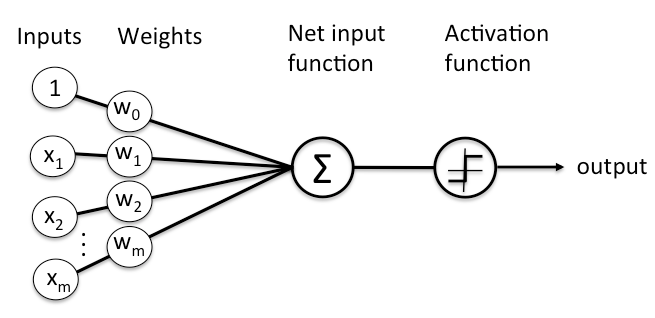
\includegraphics[width=7cm]{node_structure}
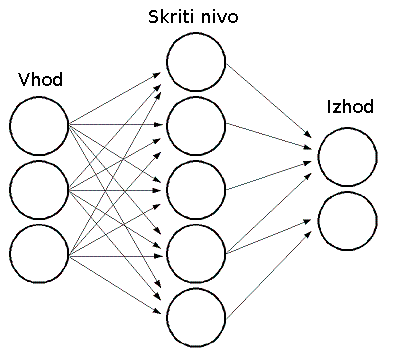
\includegraphics[width=4cm]{nn_structure}
\end{center}
\caption{Leva slika prikazuje zgradbo enega vozlišča, ki ima zasnovo podobno nevronom v možganih, desna pa zgradbo več nivojske nevronske mreže. Iz: Introduction to Deep Neural Networks url{https://deeplearning4j.org/neuralnet-overview} in Neural Networks, url{http://docs.opencv.org/2.4/modules/ml/doc/neural\_networks.html} (dostopano: 21. junij 2017)}
\label{im:nn-structure}
\end{figure}

Nivojem v nevronskih mrežah, ki se nahajajo med vhodnim in izhodnim nivojem rečemo \textit{skriti nivoji} (angl. \textit{hidden layers}). Tradicionalni algoritmi na področju strojnega učenja so sestavljeni iz vhodnega, izhodnega nivoja in enega skritega nivoja, \textit{globoka nevronska mreža} (ang. \textit{deep neural network}) pa ima po definiciji vsaj dva skrita nivoja, večinoma pa mnogo več. Vsak nivo globoke nevronske mreže prepozna določen lastnosti vhodnih podatkov. Nivoji, ki se nahajajo globje lahko prepoznajo bolj kompleksne lastnosti podatkov, saj na vhodu, dobijo lastnosti oziroma aktivacije nivoja pred njim. 

Da nevronska mreža daje zadovoljive rezultate je potrebno utežem določiti prave vrednosti. To naredimo s postopkom učenja. Vsaka nevronska mreža ima cenilno funkcijo (ang. loss function), ki pove kako dobre rezultate na testnih podatkih nevronska mreža daje trenutno. V postopku učenja zmanjšujemo vrednost cenilne funkcije z enim od algoritmov optimizacije. 

\subsection{Konvolucijske nevronske mreže}

Ker bi bilo na primeru slik pri uporabi klasičnih nevronskih mrež hitro preveč parametrov, kar bi poleg podaljšanja časa učenja povzročilo tudi prekomerno prilagajanje (ang. overfitting), uporabljamo za take primere konvolucijske nevronske mreže. Te so zelo podobne običajnim nevronskim mrežam. Sestavljene so iz nevronov, ki imajo svoje uteži in bias, ki so učljivi. Operacije znotraj nevrona so podobne tistim pri običajnih nevronskih mrežah, le da so prilagojene pričakovanim vhodnim podatkom - slikam \cite{Karpathy2016}. Vhod v vsak nivo nevronske mreže je torej matrika z obliko \textit{širina x višina x globina}. Te so v osnovi sestavljene iz treh vrst nivojev:

\begin{itemize}

\item \textbf{Konvolucijski nivo} je glavni gradnik konvolucijske nevronske mreže. Parametri tega nivoja so sestavljeni iz majhnih konvolucijskih jeder, ki pokrivajo majhno polje v širino in višino obenem pa pokrivajo celotni nivo v globino. Med prehodom po nevronski mreži izvedemo konvolucijo po celotni višini in širi vhodne matrike, po globini pa se te izhode teh konvolucij sešteje enako kot pri običajni nevronski mreži. Izhod konvolucije z enim setom jeder je dvodimenzionalna matrika. 

\item \textbf{Pooling nivo} je namenjen pod-vzorčenju (ang. downsampling) na določenem nivoju. S tem zmanjšamo število parametrov, kar vpliva zmanjšanje računske zahtevnosti in prekomernega prilagajanja. Deluje na principu, da je točna lokacija značilke manj pomembna kot približna lokacija glede na ostale značilke. 

\item \textbf{Polno povezni nivo} je nivo enak skritim nivojem pri klasični nevronski mreži. Uporabi se za zadnjih nekaj nivojev pri konvolucijski nevronski mreži. 

\end{itemize}

\section{Predstavite podatkov}
\label{se:podatki}

Slike, ki jih uporabljamo za učenje so shranjene v \textit{RGB} \cite{Pm2013} barvnem prostoru. Kot je pokazano v \cite{Iizuka2016} se izkaže, da prostor RGB ni direktno primeren za učenje algoritmov za barvanje iz dveh razlogov:

\begin{itemize}

\item \textbf{Sistem se ne ujema dobro s človeško percepcijo barv}, saj so razdalje med enako sorodnimi barvami različne glede na odtenek \cite{Prangnell}. Na primer, če imamo dva para barv rdečo in svetlo rdečo, ter modro in svetlo modro, pri čemer sta barvi v vsakem paru za človekov vizualni sistem enako različni, sta razdalji v RGB barvnem prostoru različni . 

\item \textbf{Nima kanala ločenega kanala za svetlost} Glede na to, da modeli za barvanje napovedujejo le barvne elemente v sliki, svetlost pa se vzame iz originalne slike, je najbolj priročno, če uporabljamo barvni prostor, ki ima ločen kanal za svetlost. 

\end{itemize}

\subsection{Izbira primernega barvnega prostora}

Na podlagi teh predpostavk je izbira prostorov omejena na \textit{Lab} \cite{Bansal}, \textit{YUV} in \textit{HSL} \cite{Pm2013}. Vsi ustrezajo drugi predpostavki iz \ref{se:podatki}. Edini, ki zares ustreza prvi predpostavki je \textit{Lab}. Iz ugotovitev iz sorodnih del \cite{Iizuka2016, Zhang2016, Larsson2016} se tudi najbolje izkaže prostor \textit{CIE L*a*b}.

Obstaja več verzij barvnega prostora \textit{Lab}, vendar se trenutno najbolj uporablja \textit{CIE L*a*b*}, ki naj bi bil najboljša aproksimacija človeškega vizualnega sistema \cite{Prangnell}. Prostor ima to prednost, da je neodvisen od naprave. 
Prostor CIE L*a*b* predstavi vse barve, ki jih je možno zaznati z tremi barvnimi kanali. $L*$ predstavlja svetlost, $a*$ se razširja od zelene proti rdeči barvi in $b*$ od modre proti rumeni. $L*$ ser razteza od 0, ki predstavlja črno barvo, do 100, ki predstavlja belo barvo. Prostor je grafično prikazan na sliki \ref{img:lab} $a*$ in $b*$ komponenti nimata uradne omejitve, vendar sta v implementacijah ponavadi omejene na vrednosti v intervalu $[-128, 127]$, kar je možno predstaviti z 8 bitnim celim številom. Ker zaradi pretvorb iz barvnega prostora \textit{RGB} vrednosti višje od $100$ ali nižje $-100$ redko dosežemo nekatere implementacije omejijo barvni prostor na interval $[-100, 100]$. Za pomoč pri implementaciji nevronske mreže smo sami preizkusili kakšen je dejanski interval barv pretvorjenih iz \textit{RGB} barvnega prostora. Intervale si lahko pogledate v tabeli \ref{tab:rgbcie}.

\begin{figure}
\begin{center}
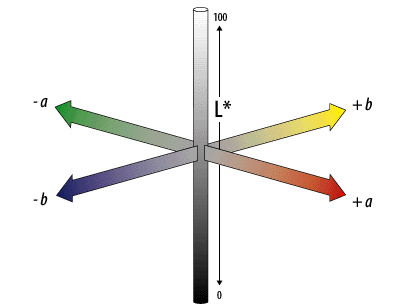
\includegraphics[width=6cm]{cielab}

\end{center}
\caption{Slika prikazuje kanale barvnega prostora CIE L*a*b*. L* predstavlja svetlost, a* se razteza od zelene barve v najbolj negativni točki proti rdeči barvi, b* ser razteza od modre proti rumeni. Nasprotujoče barve na kanalih a* in b* se nikoli ne kombinirajo v odtenek. Iz: Adobe, Technical Guid, CIELAB, \url{http://dba.med.sc.edu/price/irf/Adobe_tg/models/cielab.html} (dostopano: 24. junij 2017)}
\label{nn-structure}
\end{figure}

\begin{table}
\caption{Njavečje in njmanjše vrednosti posamezne komponente CIE L*a*b* barvnega prostora, pri pretvorbi vseh barv iz barvnega prostora RGB. Pretvorba je bila narejena z uporabo osvetlitve $D65$, ki določa temperaturo bele točke. }
\begin{center}
    \begin{tabular}{l|ccc}
        Kanal & Najmanjša vrednost & Največja vrednost \\
        \hline
        L* & 0 & 100 \\
        a* & -86.185 & 98,254 \\
        b* & -107.863 & 94.482 \\
    \end{tabular}
\end{center}
\label{tab:rgbcie}
\end{table}

\subsection{Pretvarjanje med RGB in CIE L*a*b* barvnim prostorom}

Za pretvorbo med prostoroma ni enostavne enačbe, saj je \textit{RGB} barvni prostor odvisen od naprav, \textit{CIE L*a*b*} pa ne. Tako se pretvorba zgodi v treh korakih 

\begin{enumerate}

\item \textbf{Pretvorba iz RGB v sRGB ali Adobe RGB}, saj sta ta barvna prostora neodvisna od naprave. Ta pretvorba je odvisna od naprave. Slike, ki jih bomo uporabili v našem delu so že v sRGB obliki, saj so bile pretvorjene, ko so bile zajete z fotoaparatom.

\item \textbf{Pretvorba CIE 1931 barvni prostor} ali drugače imenovan XYZ barni prostor. Ta pretvorba se izvede s pomočjo linearne pretvorbe z matriko. Matrika je odvisna od izibire referenčne bele barve. Običajno se izbere referenčno temperaturo belo točke \textit{D65}, ki je tudi standardizirana\footnotemark \cite{Ohta2005}.

\footnotetext{Zapis na uradni strani komisije International Commision on Illumination (krajše CIE), ki je postavila standard: \url{http://cie.co.at/index.php?i_ca_id=484}}

\item \textbf{Pretvorba iz XYZ v L*a*b*} se izvede po enačbah opisanih v \cite{Schwiegerling2004}.  % če je potrebno jih lahko prepišem

\end{enumerate}

\section{Obstoječe metode}

Metode za barvanje črno-belih slik delimo v dve večji skupini. Prva zahteva interakcijo uporabnika, pri drugi pa barvanje poteka popolnoma avtomatsko.

\subsection{Metode, ki zahtevajo interakcijo uporabnika}

To skupion metod delimo na tehnike, ki temeljijo na uporabnikovem barvanju manjših delov slik (ang. {\em scribble based}) \cite{levin2004colorization, huang2005adaptive} in tiste, ki temeljijo na primerih (ang. {\em example based}) \cite{Koleini2010, shirley2001color, tai2005local}. Pri prvih uporabnik določi barvo določenih točk v sliki, te pa algoritem avtomatsko razširi preko cele slike. Pri barvanju na primerih pa mora uporabnik izbrati sliko, ki je podobna tisti, ki jo želimo pobarvati, algoritem nato lastnosti izbrane slike razširi na drugo sliko ali množico slik. Tehnika barvanja s primeri se uporablja za barvanje videov, saj je v tem primeru potrebno ročno pobarvati na primer vsako stoto sliko, na ostale pa algoritem sam razširi lastnosti ročno barvane slike. 

\subsection{Popolnoma avtomatske metode}

V magistrskem delu se osredotočamo na avtomatske metode barvanja. To so algoritmi, ki samostojno, brez uporabnikovega posredovanja, obarvajo celotno sliko. Prvi dve metodi, ki sta bili predlagani na tem področju, temeljita na značilkah (ang. {\em features}) pridobljenih iz slike. Tukaj gre predvsem za značilke, ki opisujejo intenziteto posamezne barve in opisnike, ki opisujejo robove v sliki. Prva metoda uporablja za barvanje nevronsko mrežo \cite{Cheng2015}, ki pa vsebuje zgolj polnopovezane nivoje, druga pa za barvanje uporabi metodo naključnih gozdov (ang. {\em random forest}) \cite{Deshpande2015}. 

Novejši pristopi barvanja črnobelih slik tipično temeljijo na konvolucijskih nevronskih mrežah, ki imajo to lastnost, da v vsakem nivoju same odkrijejo značilke, ki so pomembni. Prva tovrstna rešitev \cite{Dahl} gradi mrežo na podlagi  že zgrajene šestnajst-nivojske mreže VGG-16, ki so jo razvili na univerzi v Oxfordu \cite{simonyan2014very}. Rešitev uporablja evklidsko cenilno funkcijo in barvni prostor YUV. Slabost te rešitve je, da izhodne barvne slike niso dovolj nasičene. 

V zadnjem času predlagane rešitve popravijo problem nenasičenosti z uporabo softmax funkcije v zadnjem nivoju nevronske mreže, kar pomeni, da so problem spremenili iz regresijskega v klasifikacijskega.  
Zang in sod. \cite{zhang2016colorful} uporabijo konvolucijsko nevronsko mrežo z več nivoji in aktivacijskimi funkcijami ReLU. Posebnost te mreže je cenilna funkcija. Uporablja križno entropijo, ki pa je v tem primeru izvedena na primerjavi barv posameznih delov slike glede na barvni prostor, ki je kvantiziran. Napake so pomnožene z utežjo, ki določa pogostost barve. Bolj redke barve so obtežene tako, da prispevajo večji delež k napaki, ki jo izračuna cenilna funkcija. S tem so avtorji izboljšali rezultate, tako da se bolj pogosto pojavljajo tudi močnejši odtenki (tisti z višjimi vrednostmi v prostoru \textit{a*b*}, ki so bili prej redkeje zastopani zaradi bolj pogostega pojavljanja nežnejših barv v slikah (barve bližje vrednostim $(0, 0)$ v \textit{a*b*} prostoru. Pogostost je bila izračunana z analizo vseh slik v podatkovni zbirki Imagenet \cite{ILSVRC15}.  Uporabljajo barvni prostor L*a*b. 
Larsson in sod. \cite{larsson2016learning} za osnovo uporabijo mrežo VGG-16, iz katere vzamejo napovedi vsakega nivoja, ki jih združijo v enotno matriko. Sledi še en polno-povezan nivo na nivoju točk v sliki. Rezultat klasifikacije je histogram za vsako točko v sliki (histogram z verjetnostmi). Uporabljajo barvni prostor HSV. Cenilna funkcija, ki jo uporabljajo je KL-divergenca, ki primerja izhodni histogram z v histogram pretvorjeno originalno sliko. 
Iizuka in sod. \cite{Iizuka2016} uporabijo nevronsko mrežo sestavljeno iz dveh delov. Prvi del poskrbi za napovedovanje vsebine slike, ki se potem združi z drugim delom in izboljša natančnost barvanja. Uporabili so križno entropijo (ang. {\em cross entropy}) v kombinaciji s cenilno funkcijo \textit{povprečna kvadratna napaka} (ang. {\em Mean squared error}) in barvni prostor L*a*b. Za razliko od prejšnjih dveh metod zadnja ne napoveduje histograma na podlagi kvantiziranega prostora ampak direktno $a*$ in $b*$ vrednost, kar pomeni, da ne uporablja klasifikacije ampak regresijo.


%----------------------------------------------------------------
% Poglavje (Chapter) 2
%----------------------------------------------------------------
\chapter{Sklicevanje na besedilne konstrukte}
\label{ch:sklicevanje}

Matematična ali popolna indukcija je eno prvih orodij, ki jih spoznamo za dokazovanje trditev pri matematičnih predmetih.
\begin{izrek}
\label{iz:1}
Za vsako naravno število $n$ velja
\begin{equation}
n < 2^n.
\label{eq:1}
\end{equation}
\end{izrek}
\begin{dokaz}
Dokazovanje z indukcijo zahteva, da neenakost~\eqref{eq:1} najprej preverimo za najmanjše naravno število --- $0$. Res, ker je $0 < 1 = 2^0$, je neenačba~\eqref{eq:1} za $n=0$ izpolnjena.

Sledi indukcijski korak. S predpostavko, da je neenakost~\eqref{eq:1} veljavna pri nekem naravnem številu $n$, je potrebno pokazati, da je ista neenakost v veljavi tudi pri njegovem nasledniku --- naravnem številu $n+1$. Računajmo.
\begin{align}
n+1 &< 2^n + 1  \label{eq:2}\\
    &\le 2^n + 2^n \label{eq:3}\\
    &= 2^{n+1} \nonumber
\end{align}
Neenakost~\eqref{eq:2} je posledica indukcijske predpostavke, neenakost~\eqref{eq:3} pa enostavno dejstvo, da je za vsako naravno število $n$ izraz $2^n$ vsaj tako velik kot 1. S tem je dokaz Izreka~\ref{iz:1} zaključen.
\end{dokaz}

Opazimo, da je \LaTeX\ številko izreka podredil številki poglavja.



%----------------------------------------------------------------
% Poglavje (Chapter) 3
%----------------------------------------------------------------
\chapter{Plovke: slike in tabele}
\label{ch:plovke}

Slike in daljše tabele praviloma vključujemo v dokument kot plovke. Pozicija plovke v končnem izdelku ni pogojena s tekom besedila, temveč z izgledom strani. \LaTeX\ bo skušal plovko postaviti samostojno, praviloma na vrh strani, na kateri se na takšno plovko prvič sklicujemo. Pri tem pa bo na vsako stran končnega izdelka želel postaviti tudi sorazmerno velik del besedila. V skrajnem primeru, če imamo res preveč plovk, se bo odločil za stran popolnoma zapolnjeno s plovkami.

\section{Formati slik}
Bitne slike, vektorske slike, kakršnekoli slike, z \LaTeX{}om lahko vključimo vse.
Slika~\ref{pic1} je v {\tt .pdf} formatu.
\begin{figure}
    \begin{center}
        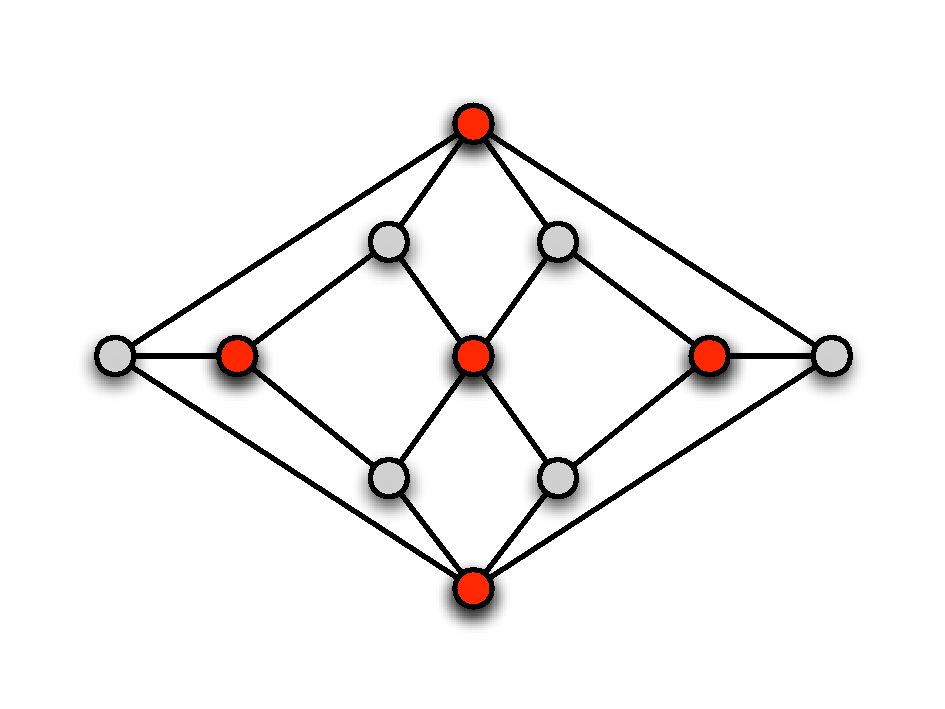
\includegraphics[width=10cm]{pic1.pdf}
    \end{center}
\caption{Herschelov graf, vektorska grafika.}
\label{pic1}
\end{figure}
Pa res lahko vključimo slike katerihkoli formatov? Žal ne. Programski paket \LaTeX\ lahko uporabljamo v več dialektih. Ukaz {\tt latex} ne mara vključenih slik v formatu Portable Document Format {\tt .pdf}, ukaz {\tt pdflatex} pa ne prebavi slik v Encapsulated Postscript Formatu {\tt .eps}.
Strnjeno v Tabeli~\ref{tbl:1}.

\begin{table}
\caption{}
    \begin{center}
        \begin{tabular}{l|ccc}
            ukaz/format & {\tt .pdf} & {\tt .eps} & ostali formati \\ \hline
                        {\tt pdflatex} & da & ne & da \\
                        {\tt latex}   & ne & da  & da
        \end{tabular}
    \end{center}
\label{tbl:1}
\end{table}

Nasvet? Odločite se za uporabo ukaza {\tt pdflatex}. Vaš izdelek bo brez vmesnih stopenj na voljo v {.pdf} formatu in ga lahko odnesete v vsako tiskarno. Če morate na vsak način vključiti sliko, ki jo imate v {\tt .eps} formatu, jo vnaprej pretvorite v alternativni format, denimo {\tt .pdf}.

Včasih se da v okolju za uporabo programskega paketa \LaTeX\ nastaviti na kakšen način bomo prebavljali vhodne dokumente. Spustni meni na Sliki~\ref{pic2} odkriva uporabo \LaTeX{}a v njegovi pdf inkarnaciji --- {\tt pdflatex}.
\begin{figure}
\begin{center}
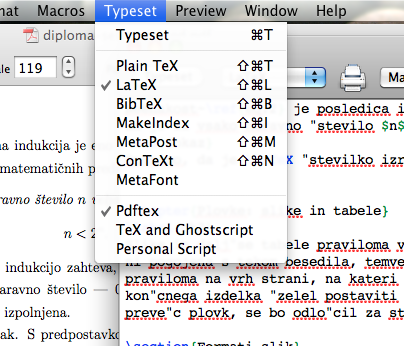
\includegraphics[width=10cm]{pic2.png}
\end{center}
\caption{Kateri dialekt uporabljati?}
\label{pic2}
\end{figure}
Vključena Slika~\ref{pic2} je seveda bitna.



%----------------------------------------------------------------
% Poglavje (Chapter) 4
%----------------------------------------------------------------
\chapter{Razno}
\label{ch:razno}

\section{Notacije}
\label{sec:notacije}

Za notacijo spremenljivk ter skalarjev uporabimo običajno notacijo, t.j., spremenljivka $x$ in skalar $a$. Pri notaciji matrik ter vektorjev pa se poslužujemo krepega fonta. Torej, matrika $\boldsymbol{A}$ ter vektor $\boldsymbol{v}$,
\begin{equation}
\boldsymbol{A} = \begin{bmatrix}
       a_{11} & a_{12} & \dots & a_{1q}  \\
       a_{21} & a_{22} & \dots & a_{2q}  \\
       \vdots  \\
       a_{p1} & a_{p2} & \dots & a_{pq}  \\
     \end{bmatrix}, \quad
     \boldsymbol{v} = \begin{bmatrix}
       x_1  \\
       x_2  \\
       \vdots  \\
       x_q  \\
     \end{bmatrix}. \nonumber
\end{equation}

%----------------------------------------------------------------
\section{Lepe tabele in psevdokoda}
\label{sec:psevdokoda}

Psevdokoda~\ref{alg:primer} prikazuje primer delovanja genetskega algoritma, medtem ko Tabela~\ref{tab:params} prikazuje primer lepe tabele brez vertikalnih črt.

\begin{algorithm}
\caption{Psevdokoda genetskega algoritma}
\label{alg:primer}
\begin{algorithmic}[1]
\footnotesize
\STATE $t \gets 0$
\STATE $InitPopulation[P(t)] \gets$ inicializiraj populacijo
\STATE $EvalPopulation[P(t)] \gets$ evaluiraj populacijo
\REPEAT
\STATE $P'(t) \gets Variation[P(t)] \gets $ generiraj novo populacijo
\STATE $EvalPopulation[P'(t)] \gets$ evaluiraj novo populacijo
\STATE $P(t+1) \gets ApplyGeneticOperators[P'(t) \in Q]$
\STATE $t \gets t+1$
\UNTIL{prekinitev}
\IF{rezultat dovolj dober}
\STATE shrani rezultat
\ENDIF
\end{algorithmic}
\end{algorithm}

%---------------------------------------------------------------
\begin{table}
\caption{Primer enostavne tabele.}
\centering
\scalebox{0.82}{
\begin{tabular}{c c c}
 \toprule
 Ime & Vrednost & Opis \\
 \midrule
 \textit{ $a$ } & 0.03 &  skalar \\
 \textit{ $x$ } & -1 & spremenljivka \\
 \bottomrule
\end{tabular}
}
\label{tab:params}
\end{table}

%----------------------------------------------------------------
% Poglavje (Chapter) 5
%----------------------------------------------------------------
\chapter{Kaj pa literatura?}
\label{ch3}
Kot smo omenili že v uvodu, je pravi način za citiranje literature uporaba \BibTeX{}a~\cite{ubi}.
Programski paket \LaTeX je prvotno predstavljen v priročniku~\cite{Lamport} in je v resnici nadgradnja sistema \TeX\ avtorja Donalda Knutha, znanega po denimo, če izpustim njegovo umetnost programiranja, Knuth-Bendixovem algoritmu~\cite{Knuth}.

Vsem raziskovalcem s področja računalništva pa svetujem v branje mnenje L.\ Fortnowa~\cite{Fortnow}.

%----------------------------------------------------------------
% Poglavje (Chapter) 6
%----------------------------------------------------------------
\chapter{Sklepne ugotovitve}
Izbira \LaTeX\ ali ne \LaTeX\ je seveda prepuščena vam samim. Res je, da so prvi koraki v \LaTeX{}u težavni. Ta dokument naj vam služi kot začetna opora pri hoji.

% ---------------------------------------------------------------
% Appendix
% ---------------------------------------------------------------
\appendix
%\addcontentsline{toc}{chapter}{Razširjeni povzetek}
\chapter{Title of the appendix 1}

Example of the appendix.

%----------------------------------------------------------------
% SLO: bibliografija
% ENG: bibliography
%----------------------------------------------------------------
\bibliographystyle{elsarticle-num}

%----------------------------------------------------------------
% SLO: odkomentiraj za uporabo zunanje datoteke .bib (ne pozabi je potem prevesti!)
% ENG: uncomment to use .bib file (don't forget to compile it!)
%----------------------------------------------------------------
%\bibliography{bibliography}

%----------------------------------------------------------------
% SLO: zakomentiraj spodnji del, če uporabljaš zunanjo .bib datoteko
% ENG: comment the part below if using the .bib file
%----------------------------------------------------------------

\begin{thebibliography}{99}
\bibitem{Fortnow} L.\ Fortnow, ``Viewpoint: Time for computer science to grow up'',
{\it Communications of the ACM}, št.\ 52, zv.\ 8, str.\ 33--35, 2009.
\bibitem{Knuth} D.\ E.\ Knuth, P. Bendix. ``Simple word problems in universal algebras'', v zborniku: Computational Problems in Abstract Algebra (ur. J. Leech), 1970, str. 263--297.
\bibitem{Lamport} L.\ Lamport. {\it LaTEX: A Document Preparation System}. Addison-Wesley, 1986.
\bibitem{ubi} O.\ Patashnik (1998) \BibTeX{}ing.
Dostopno na: \url{http://ftp.univie.ac.at/packages/tex/biblio/bibtex/contrib/doc/btxdoc.pdf}
\bibitem{licence} licence-cc.pdf. Dostopno na: \url{https://ucilnica.fri.uni-lj.si/course/view.php?id=274}
\end{thebibliography}

\end{document}
